%%%%%%%%%%%%%%%%%%%%%%%%%%%%%%%%%%%%%%%%%%%%%%%%%%%%%%%%%%%%%%%%%%%%%%%%
%    INSTITUTE OF PHYSICS PUBLISHING                                   %
%                                                                      %
%   `Preparing an article for publication in an Institute of Physics   %
%    Publishing journal using LaTeX'                                   %
%                                                                      %
%    LaTeX source code `ioplau2e.tex' used to generate `author         %
%    guidelines', the documentation explaining and demonstrating use   %
%    of the Institute of Physics Publishing LaTeX preprint files       %
	%    `iopart.cls, iopart12.clo and iopart10.clo'.                      %
%                                                                      %
%    `ioplau2e.tex' itself uses LaTeX with `iopart.cls'                %
%                                                                      %
%%%%%%%%%%%%%%%%%%%%%%%%%%%%%%%%%%
%
%
% First we have a character check
%
% ! exclamation mark    " double quote  
% # hash                ` opening quote (grave)
% & ampersand           ' closing quote (acute)
% $ dollar              % percent       
% ( open parenthesis    ) close paren.  
% - hyphen              = equals sign
% | vertical bar        ~ tilde         
% @ at sign             _ underscore
% { open curly brace    } close curly   
% [ open square         ] close square bracket
% + plus sign           ; semi-colon    
% * asterisk            : colon
% < open angle bracket  > close angle   
% , comma               . full stop
% ? question mark       / forward slash 
% \ backslash           ^ circumflex
%
% ABCDEFGHIJKLMNOPQRSTUVWXYZ 
% abcdefghijklmnopqrstuvwxyz 
% 1234567890
%
%%%%%%%%%%%%%%%%%%%%%%%%%%%%%%%%%%%%%%%%%%%%%%%%%%%%%%%%%%%%%%%%%%%
%
\documentclass[12pt]{iopart}
\newcommand{\gguide}{{\it Preparing graphics for IOP Publishing journals}}

%Uncomment next line if AMS fonts required
%\usepackage{iopams}  
\usepackage{amsfonts}
\usepackage{amssymb}
\usepackage{xcolor}
\usepackage{color}
\usepackage{pdfpages}
\usepackage{float}
\usepackage{multirow}
\usepackage{multicol}
\usepackage{amsbsy}
\usepackage[none]{hyphenat}
\usepackage{footnote}
\usepackage{tabularx}
\usepackage{epstopdf}
\usepackage{setspace} % for double spacing, maybe remove later
\usepackage{mathrsfs} 
\usepackage[hyphens]{url}
\usepackage[english]{babel}
\usepackage{harvard}
\usepackage[flushleft]{threeparttable}
\usepackage{changepage}


\begin{document}

\pdfminorversion=4
\submitto{\ERL}
\makesavenoteenv{tabular}

\title{The Effects of weather on maize yields: New evidence from Kenya}

\author{Monika Novackova, Pedram Rowhani, Martin Todd and Dominic Kniveton}

\address{Department of Geography, University of Sussex, Falmer, UK}
\ead{monika.novac@gmail.com}
\vspace{10pt}
\begin{indented}
\item[]November 2018
\end{indented}

\doublespacing
\begin{abstract}
...Applying the linear mixed effects models, we found that...\\
\textcolor{blue}{.. to be written later..}
\end{abstract}

%
% Uncomment for keywords
%\vspace{2pc}
%\noindent{\it Keywords}: XXXXXX, YYYYYYYY, ZZZZZZZZZ
%
% Uncomment for Submitted to journal title message
%\submitto{\JPA}
%
% Uncomment if a separate title page is required
%\maketitle
% 
% For two-column output uncomment the next line and choose [10pt] rather than [12pt] in the \documentclass declaration
%\ioptwocol
%
\maketitle
\section{Introduction}\label{Introduction}


\begin{itemize}
\color{blue}
\item[] \textbf{Paragraph 1}

\begin{itemize}

\item Extreme weather causes disasters $\rightarrow$	 early warning systems have been developed
\end{itemize}
\item[] \textbf{Paragraph 2}
\begin{itemize}
\item What weather forecasts (measures) have been used in EWS? \textit{ref. litrature}
\begin{itemize}
\item Mostly seasonal precip. totals and temperature averages
\end{itemize}
\end{itemize}

\item[] \textbf{Paragraph 3} 
\begin{itemize}

\item Identify difference between hazard and disaster

\begin{itemize}
\item Not every hazard turns into disaster
\item For a hazard to become a disaster it needs to have \textbf{impact}
\item Here, we identify the key metrics which have impact on yield
\end{itemize}

\end{itemize}

\item[] \textbf{Paragraph 4}
\begin{itemize}
\item Crop yield versus climate forecasting
\end{itemize}


\item[] \textbf{Paragraph 5}
	\begin{itemize}
		\item Aim of the paper
		\end{itemize}
	 
	\end{itemize}





\section{Methods}\label{Methods}
\color{blue}

...a case study looking at Kenya...
\color{black}

Our dataset consists of an yearly panel of $47$ counties of Kenya describing the period of 1981-2017.
 
\subsection{Data}\label{Data}
\color{blue}
\begin{itemize}
\item Source of the climate data: BOKU and Berkeley Earth
\item Source of the yield data (Kenya MoA)
\end{itemize}

\color{black}
\subsection{Statistical approach}

% No need to write too many details (or a section) about measures of food security
% No need to describe all the weather measures/characteristics that we have calculated and/or tried to use and didn't work
\begin{itemize}
\color{blue}
\item \textit{We used commonly used measures of weather/drought (Only mention the significant weather measures/variables)}
\item Describe the temporal aggregation of the weather variables, seasons
\end{itemize}
\color{black}

\sloppy
Kenya consists of $47$ counties with semi-autonomous county governments  \cite{Barasa2017}. As a result of the high degree of county-level autonomy, the policies and regulations often differ across the counties, hence the effects of weather on crop yield are likely to be different across the counties. Therefore, following the standard methodology, we estimated a battery of linear mixed effects models (also known as mixed models) commonly used to analyse longitudinal data \cite{bates2000mixed}. Mixed models are suitable for analysis of panel data as they account for the panel structure of the dataset. These types of models include both fixed effects parameters and random effects. Fixed effects are analogous to parameters in a classical linear regression model and value of each effect is assumed to be fixed over all counties \cite{bates2010lme4}. On the other hand, random effects are unobserved random variables. There are at least three benefits of treating a set of parameters as a random sample from some distribution. \textit{(i)} Extrapolation of inference to a wider population \textit{(ii)} improved accounting for system uncertainty and \textit{(iii)} efficiency of estimation %(\citealp{KERYch9, KERYch12}).

Formally, a linear mixed model can be described by the distribution of two vectors of random variables: the response $\mathscr{Y}$ and the vector of random effects $\mathscr{B}$. The distribution of $\mathscr{B}$ is multivariate normal and the conditional distribution of $\mathscr{Y}$ given $\mathscr{B}=\mathbf{b}$ is multivariate normal of a form %(\citealp{bates2010lme4, KERYch9}):




\begin{equation}\label{MixedGeneral}
\begin{array}{lcl}

(\mathscr{Y}|\mathscr{B}=\mathbf{b})& \sim & \mathit{N}(\mathbf{X}\mathbf{\beta}+\mathbf{Z}\mathbf{b},\sigma^2\mathbf{I}),

\end{array}
\end{equation}

where $\mathbf{X}$ is an $n \times p$ model matrix of fixed effects, $\mathbf{\beta}$ is a $p$-dimensional fixed-effects parameter, $\mathbf{Z}$ is an $n \times q$ model matrix for the $q$-dimensional vector of random-effects variable $\mathscr{B}$ evaluated at $\mathbf{b}$ and $\sigma$ a scale factor. The distribution of $\mathscr{B}$ can be written as: 

\begin{equation}\label{ranefDist}
\mathscr{B} \sim \mathit{N}(0,\mathbf{\Sigma}),
\end{equation}

where $\mathbf{\Sigma}$ is a $q \times q$ positive semi-definite variance-covariance matrix.

\color{blue}
\begin{itemize}
\item Add a description of residual and other diagnostic tests (AIC, VIF, autocorrelation)
\item Describe the procedure that I have applied to find the preferred combination of fixed effects and random effects
\item Describe the procedure that I have applied to find the preferred way of modelling the  correlation structure in errors (ARMA errors)
\end{itemize}
\color{black}





	\section{Results}\label{Results}

\color{blue}
\begin{itemize}

\item Tables of estimates of the preferred specification which includes the significant weather variables (see the preliminary results in Table \ref{KenARe11}) 

\begin{itemize}
\item For all counties 
\item For Arid and semi-araid (ASAL) counties
\item For non-ASAL counties
\end{itemize}

\color{black}

{
\begin{threeparttable}
\singlespacing
\caption{\textit{\textbf{Mixed  effects model:} Log of maize yield and weather, ARMA(1,1) errors}}
%KEN11a  KEN11a_ASAL    KEN11a_nonASAL														
\label{KenARe11} 
\begin{footnotesize}
\begin{tabular}{llrlllr} 
\hline \vspace{-0.2cm} \\
\vspace{-0.2cm} \\
  \multicolumn{1}{l}{\vspace{0.1cm}\textbf{ }}  &\multicolumn{2}{c}{\textit{\textbf{All counties}}} &\multicolumn{2}{c}{\textit{\textbf{ASAL}}} &\multicolumn{2}{c}{\textit{\textbf{non-ASAL}}}\\
    \multicolumn{1}{l}{\vspace{0.1cm}\textbf{Fixed effects:}}&{$exp(\beta)$}&\textbf{F-value\tnote{a}}% anova(KEN11a, type='marginal')
    &{$exp(\beta)$}&\textbf{F-value\tnote{a}}&{$exp(\beta)$}&\textbf{F-value\tnote{a}}\\
 \hline 
\hline
\\
\vspace{-0.2cm}Intercept&$1.296^{***}$&$19.916$&$1.276^{*}$&$5.230$&$1.410^{**}$&$10.061$\\
  \\ \vspace{-0.2cm}Prec. total&$1.081^{*}$&$5.402$&$1.006^{}$&$0.022$&$1.278^{***}$&$19.386$\\
  \\
  \vspace{-0.2cm}Prec. total sq.&$0.973^{*}$&$4.289$&$1.004$&$0.051$&$0.880^{***}$&$23.747$\\
    \\ \vspace{-0.2cm}Prec. c. of var.&$0.924^{\bullet}$&$3.277$&$0.969$ &$0.246$&$0.909^{}$&$2.231$\\
  \\  \vspace{-0.2cm}Dry spell -length&$0.935^{*}$&$4.810$&$0.833^{**}$&$6.969$&$ 0.988^{}$&$0.163$\\
  \\ \vspace{-0.2cm}Dry spells 	$\geq$ 4 d.&$0.939^{*}$&$4.826$&$0.855^{**}$&$8.065$&$0.989^{}$&$0.096$\\
  \\ \vspace{-0.2cm}Temp. - average&$0.819^{***}$&$12.127$&$0.808^{*}$&$5.376$&$0.878$ $^{}$&$1.580$\\
  \\  \vspace{-0.2cm}Temp. std. dev.&$1.043^{\bullet}$&$3.125$&$1.039$&$0.558$&$1.059$ ${*}$&$5.640$\\
  \\
  \hline
\vspace{-0.2cm} \\
  \multicolumn{1}{l}{\textbf{Random effects:}}  & \\
\vspace{-0.2cm}
\\
\hline
\\
  \vspace{-0.2cm}Intercept\\
 \\ 
 \hline
\vspace{-0.2cm} \\
\textit{Number of observations:}  &\multicolumn{2}{c}{$1300$}&\multicolumn{2}{c}{$698$}&\multicolumn{2}{c}{$602$}\\
\vspace{-0.2cm}
\\  
  
  \hline
  \vspace{-0.2cm} \\

\hline
\vspace{-0.2cm}
\end{tabular} 
\end{footnotesize}
 \begin{tablenotes}
  \begin{footnotesize}
    \item \textit{Notes:} Standard errors in brackets; \hfill $^{\bullet}~p<0.1$; $^{*}~p<0.05$; $^{**}~p<0.01$; $^{***}~p<0.001$
        \begin{adjustwidth}{1cm}{} 
    \item[a] Marginal (type III) sum of squares. The F-statistics correspond to the sum of squares attributable to each fixed effect.
     \end{adjustwidth}
\singlespacing
  \end{footnotesize}
\end{tablenotes}
  \end{threeparttable} 
\par}
\linespread{1}

  \begin{figure}
   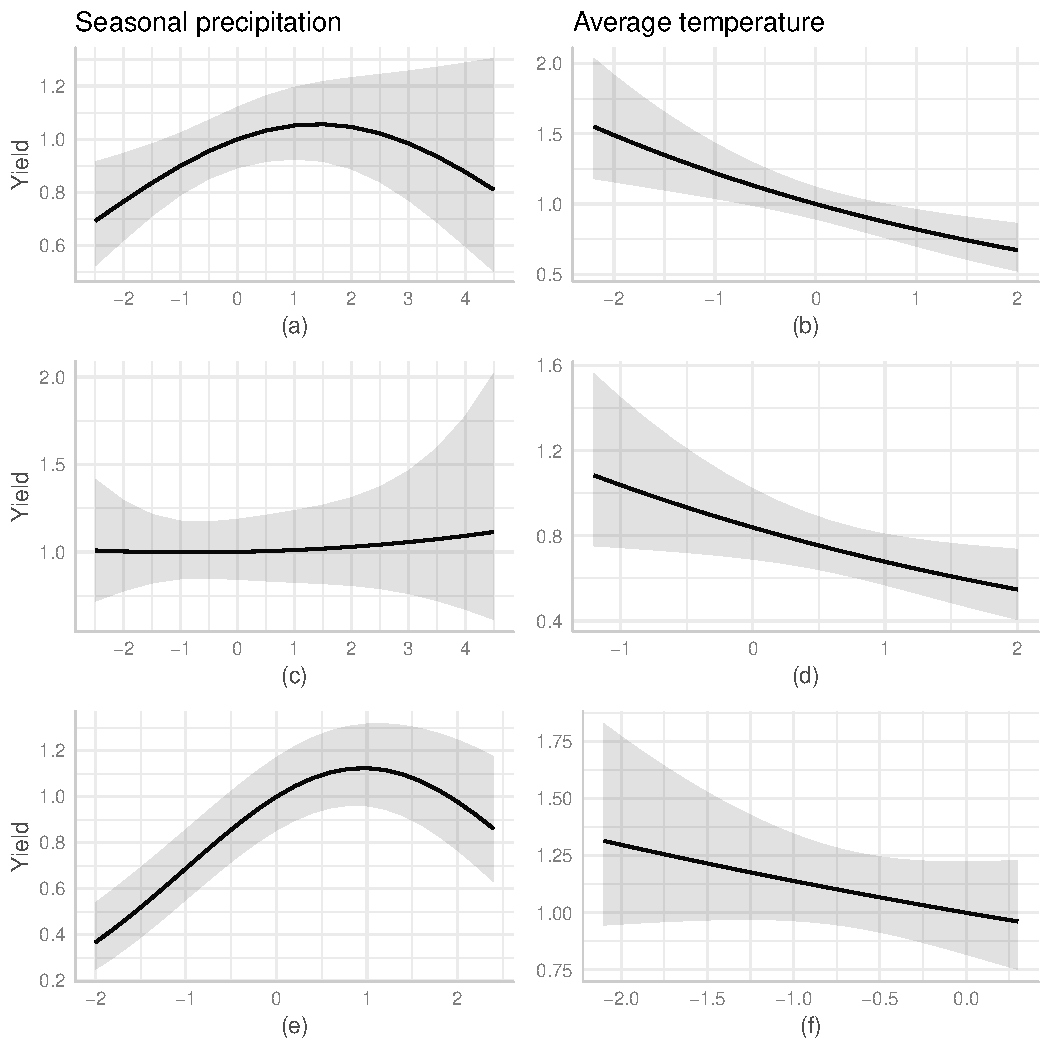
\includegraphics{Figure1a_1f.pdf}\label{bar}
\caption{Predicted multiplicative marginal effects of seasonal precipitation (left column) and average seasonal temperature (right column) on maize yields. The first row (a, b) represents the model for all counties, the second row (c, d) is based on the subsample of arid and semi-arid counties (ASAL) and the third row (e, f) represents the model for the non-ASAL counties. Precipitation and temperature (x-axis) are in multiples of their standard deviations. The effects are multiplicative as the models are in log-linear form.}
\end{figure}


  \begin{figure}
   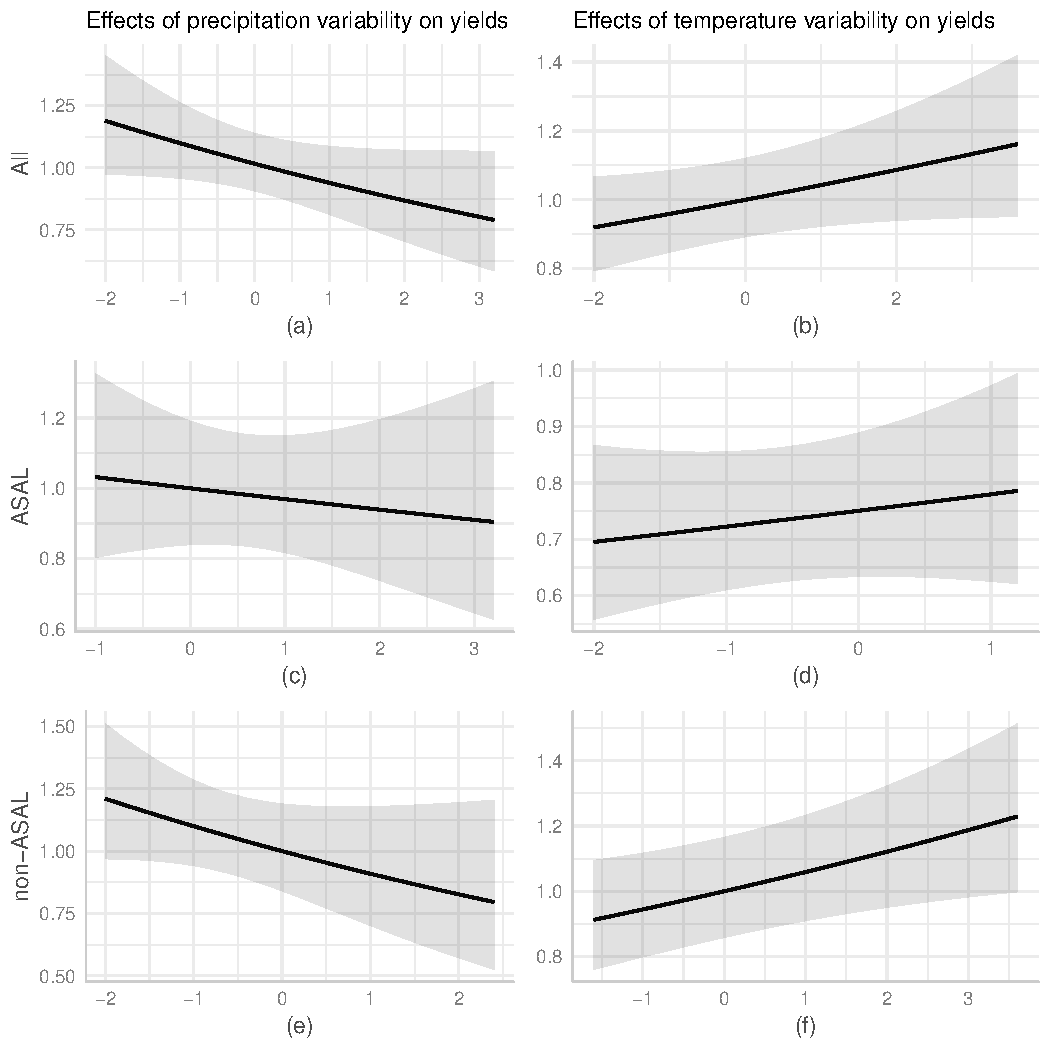
\includegraphics{Figure2a_2f.pdf}\label{bar}
\caption{Predicted multiplicative marginal effects of coefficient of variation (CV) of precipitation (left column) and standard deviation (SD) of temperature (right column) on maize yields. The first row (a, b) represents the model for all counties, the second row (c, d) is based on the subsample of arid and semi-arid counties (ASAL) and the third row (e, f) represents the model for the non-ASAL counties. CV of precipitation and SD of temperature (x-axis) are in multiples of their standard deviations. The effects are multiplicative as the models are in log-linear form.}
\end{figure}

\color{blue}

\item Verbal description and interpretation of the results. Discussing goodness of fit using various criteria such as AIC or alternatives to $R^2$.
%\item Possibly estimate simple regressions with the same explanatory variables as the preferred mixed effects specification. This would give us an approximation of $R^2$ which could be used to compare our models.

	%	\begin{itemize}%
		%	\item \textcolor{red}{Annemie has advised me that for a more precise approximation of $R^2$ we can estimate a simple regression of yields on the random intercepts (county level dummy variables) and then subtract the $R^2$ of this model from the $R^2$ of the simple regression with the explanatory variables of the preferred mixed models (the model described in the bullet point above). This would give us a percentage of yield variability explained by the weather measures not including the variability explained by the random intercepts.}
	%\end{itemize}
	
\item If we get the yield data for the period from $2015$ onwards: Out of sample predictions and comparison with the real data
\end{itemize}





\color{black}

\clearpage

\appendix
\section*{Appendix}
should be at the end of the main text but before list of references


\bibliographystyle{dcuM}

 \nocite{BOKU} 
 \nocite{Berkeley} 
\bibliography{referencesFS}

\end{document}

